\section{Análise de resposta em frequência de redes }

Distorções na rede elétrica pode ser oriunda da saturação de transformadores, circuitos retificadores (CA-CC), compensadores estáticos (bancos de capacitores ou reatores) ou até fornos a arco.

A análise é feita a partir da decomposição da onda distorcida em série de Fourier, permitindo analisar suas harmônicas. Isso é feito por meio das matrizes admitância e impedância aplicadas no ponto de frequência desejada.

A modelagem da rede leva em conta os seguintes componentes: linhas, geradores, transformadores, reatores, capacitores e cargas.

Por meio de análises anteriores para o circuito $\pi$ de uma linha longa, tem-se a seguinte matriz de admitâncias:

\begin{equation} \label{slide:4:1}
    Y\, = \,\frac{1}{Z_c senh(\gamma l)}\begin{bmatrix} cosh(\gamma l) & -1 \\ -1 & cosh(\gamma l)   \end{bmatrix}
\end{equation}

A inversão dessa matriz permite encontrar a matriz impedância $Z_{barra}$.

\subsection{Efeitos da circulação de harmônicas}

A distorção harmônica de tensão procura analisar a circulação de harmônicas de uma rede por meio de um sinal decomposto em série de Fourier. Assim, a distorção harmônica total é mensurada pelo DHT:

\begin{equation} \label{slide:4:2}
    DHT = \sqrt{\sum_{h = 2}^{50}  \left(\frac{V_h}{V_1}\right)^2}
\end{equation}

De forma que $V_1$ é o valor eficaz da fundamental e $V_h$ o valor eficaz da harmônica para $h$ maiores que a unidade (para não confundir com a fundamental). Assim o DHT vai mostrar o quão relevante as componentes harmônicas estão em comparação com a fundamental e quanto maior seu valor, maior influência de harmônicas.

\subsection{Filtragem de harmônicas}

A obtenção da resposta em frequência da rede é fundamental para o projeto de filtros de harmônicas. Para o estudo de filtros é utilizado o seguinte modelo de rede:

\begin{figure}[H]
\begin{center}
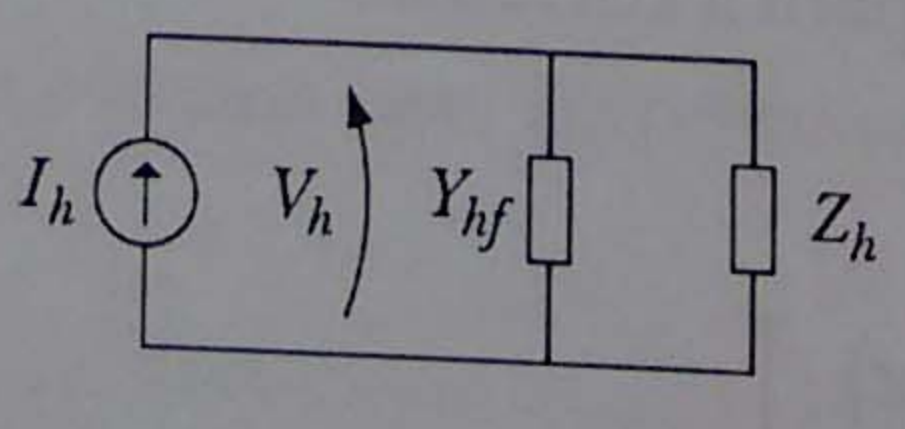
\includegraphics[width=8cm]{images/harmonicas.png}
\caption{Rede elétrica e filtro.}
\label{slide3:filt} 
\end{center}
\end{figure}

De forma que $I_h$ é a corrente harmônica injetada; $V_h$ a tensão harmônica; $Z_h$ a impedância da rede avaliada na harmônica desejada; e $Y_{hf}$ é a admitância do filtro para a harmônica desejada.

A filosofia de projeto do filtro busca um filtro que seja quase um circuito aberto do ponto de vista da corrente injetada, pois isso significaria uma tensão harmônica nula. O filtro é projetado para que isso ocorra na frequência nominal da rede e que a impedância gerada minimize a tensão harmônica de acordo com o seguinte divisor de tensão:

\begin{equation} \label{slide4:filter}
    V_h = \frac{I_h}{Y_{hf} + Y_h}
\end{equation}

Porém a associação paralela de filtros é dificultada, pois:

\begin{itemize}
    \item A configuração da rede é variável devido a  chaveamentos e dificuldade de representar as cargas no domínio da frequência;
    \item As correntes harmônicas são sujeitas a processos aleatórios;
    \item Otimização dos filtros visto sua iteração com a rede;
\end{itemize}






exemplo 14, 16, 17